\documentclass[11pt,a4paper]{article}

% ---- Packages ----
\usepackage[utf8]{inputenc}
\usepackage[T1]{fontenc}
\usepackage{geometry}
\geometry{margin=1in, top=1.2in, bottom=1.2in}
\usepackage{microtype}
\usepackage{times}
\usepackage{amsmath, amssymb}
\usepackage{graphicx}
\usepackage{booktabs}
\usepackage{natbib}
\bibliographystyle{plainnat}
\usepackage{hyperref}
\hypersetup{
  colorlinks=true,
  linkcolor=black,
  citecolor=blue,
  urlcolor=blue
}
\usepackage{caption}
\captionsetup{font=small, labelfont=bf}
\usepackage{float}
\usepackage{enumitem}
\usepackage{fancyhdr}
\pagestyle{fancy}
\fancyhf{}
\fancyhead[L]{\small STP-Diff: Differentiable Adversarial Discovery of Regulatory Vulnerabilities}
\fancyhead[R]{\small Khalil}
\fancyfoot[C]{\thepage}
\renewcommand{\headrulewidth}{0.4pt}
\usepackage{array}
\usepackage{multirow}
\usepackage{algorithm}
\usepackage{algpseudocode}
\usepackage{amsthm}
\usepackage{bm}
\newtheorem{theorem}{Theorem}[section]

% ---- Title ----
\title{\Large \textbf{STP-Diff: Differentiable Adversarial Discovery of\\[2pt] Regulatory Vulnerabilities in Gene Circuits via\\[2pt] Semi-Tensor Product Mapping}}

\author{\textbf{Yaseen Khalil}\\[4pt]
\textit{Virginia Tech Researcher}\\[2pt]
\href{mailto:yaskhalil2006@vt.edu}{yaskhalil2006@vt.edu}\\[4pt]
\href{https://github.com/yaskhalil/STP-Diff}{\texttt{github.com/yaskhalil/STP-Diff}}}

\date{}

% ---- Document ----
\begin{document}

\maketitle
\thispagestyle{fancy}

\begin{abstract}
\noindent
The discovery of regulatory vulnerabilities in Gene Regulatory Networks (GRNs) is central to computational oncology, yet remains computationally intractable for networks exceeding 15--20 nodes due to exponential state-space explosion. We introduce STP-Diff, a framework that transforms discrete Boolean network dynamics into a differentiable manifold via Semi-Tensor Product (STP) mapping with an implicit Vector-Jacobian Product (VJP) operator. This reduces theoretical complexity from $O(4^N)$ to $O(N \cdot 2^N)$, with a measured $1\,637\times$ speedup at $N=15$ (wall-clock, including explicit matrix construction) and a theoretical bound of $52\,429\times$ at $N=20$. Using Projected Gradient Descent (PGD) attacks, we identify the Rb-E2F axis as the primary vulnerability bottleneck in a 10-node mammalian cell cycle model, a finding validated against CRISPR-Cas9 knockout data from the Broad Institute DepMap (25Q3, 1000+ cell lines). We further quantify network resilience through Epsilon-Critical search, establishing $\epsilon_{\text{critical}} \approx 2.80$ for the p53-Mdm2 DNA-damage circuit. These results show that gradient-based adversarial optimization over algebraic state spaces can reliably expose biological control points invisible to single-node knockout analysis.
\end{abstract}

\section{Introduction}
\label{sec:intro}

The study of Gene Regulatory Networks (GRNs) has deep roots in dynamical systems theory. Jacob and Monod's operon model established the paradigm of logical regulation, later formalized by Kauffman~\cite{kauffman1969metabolic} into Random Boolean Networks (RBNs) and refined by Thomas~\cite{thomas1973boolean} into the logical formalism that underpins modern systems biology. Glass and Kauffman~\cite{glass1973logical} showed that even simple Boolean idealizations of biochemical networks could reproduce complex dynamical behaviors like limit cycles and multiple steady states. Albert and Othmer~\cite{albert2003topology} later demonstrated that these discrete models could make experimentally testable predictions about real biological systems, specifically the segment polarity gene network in \textit{Drosophila}.

Boolean Network (BN) models capture the switch-like behavior of gene activation: each gene is ON (1) or OFF (0), and its next state is a deterministic Boolean function of its regulators' current states. Despite their conceptual clarity, BNs face a fundamental computational barrier. The state space of an $N$-node network scales as $2^N$, and brute-force attractor analysis enumerating all possible transitions becomes intractable beyond $N \approx 15$.

Two dominant approaches have emerged to manage this complexity:

\textbf{Differential Equation (ODE) models} replace discrete logic with continuous concentration dynamics, enabling numerical simulation. However, ODEs introduce dozens of free parameters (Michaelis constants, degradation rates, Hill coefficients) that must be measured or fit, and small parameter changes can produce qualitatively different attractor landscapes~\cite{aldridge2006physicochemical}. For most biological circuits, these parameters are unknown.

\textbf{Semi-Tensor Product (STP) methods}, pioneered by Cheng et al.~\cite{cheng2011analysis}, provide an algebraic alternative. By representing Boolean states as canonical vectors in $\mathbb{R}^2$ and using the semi-tensor product in place of the standard matrix product, any Boolean network can be expressed as a linear system:
\begin{equation}\label{eq:stp_linear}
x(t+1) = L x(t),
\end{equation}
where $L \in \mathbb{R}^{2^N \times 2^N}$ is the global transition matrix. This enables algebraic control theory for network analysis and intervention design~\cite{cheng2010controllability}. However, constructing $L$ explicitly requires $O(4^N)$ memory, the ``matrix explosion'' problem, limiting practical application to $N \lesssim 10$.

\textbf{Graph Neural Networks (GNNs)} have been applied to drug response prediction~\cite{kipf2017semi} and cell-line sensitivity analysis. Standard message-passing architectures aggregate neighborhood information in ways that wash out the strict Boolean logic governing individual gene transitions. LogicXGNN~\cite{geng2026logicxgnn} attempts to bridge this gap by extracting logical rules from trained GNNs, but does not provide a mechanism for discovering vulnerabilities through optimization.

\textbf{Probabilistic Boolean Networks (PBNs)}~\cite{shmulevich2002probabilistic} introduced stochasticity to address deterministic BN limitations, but their inference problem scales exponentially with network size and does not offer a gradient-based intervention design pathway.

\textbf{This paper presents STP-Diff}, which synthesizes elements from each paradigm. The contributions are:
\begin{enumerate}[leftmargin=*]
    \item An implicit Vector-Jacobian Product (VJP) operator that computes gradients through STP networks in $O(N \cdot 2^N)$ time and $O(2^N)$ memory, avoiding explicit construction of the global transition matrix.
    \item A Temperature-Scaled Softmax relaxation that renders Boolean dynamics differentiable, enabling gradient-based adversarial attack.
    \item The first demonstration, to our knowledge, of adversarial vulnerability discovery in biological networks, validated against empirical CRISPR-Cas9 knockout data.
\end{enumerate}

\section{Problem Statement}
\label{sec:problem}

Let $G = (V, E)$ be a GRN with $N = |V|$ nodes. Each node $v_i \in V$ has a Boolean state $x_i(t) \in \{0, 1\}$ and a transition function $f_i: \{0,1\}^{k_i} \to \{0,1\}$, where $k_i$ is the in-degree of $v_i$. The global state at time $t$ is $x(t) \in \{0,1\}^N$.

The \textbf{regulatory vulnerability problem} is: given a target phenotype $s^* \in \{0,1\}^N$ (e.g., apoptosis, G1-arrest), find the minimal perturbation to the network's logical structure such that the attractor landscape shifts to include $s^*$ as a reachable fixed point.

In the Boolean setting, a perturbation corresponds to flipping one or more entries of the structure matrices $M_i$ that encode $f_i$. Brute-force evaluation of all possible perturbations requires $O(2^N \cdot |E|)$ simulations, prohibitive for $N > 10$.

We reformulate this as an adversarial optimization problem: given a baseline network $\Theta^{(0)}$, find $\Delta\Theta$ within an $\ell_\infty$ ball of radius $\epsilon$ that maximizes the probability of the target state after $T$ steps:
\begin{equation}\label{eq:adversarial_objective}
\max_{\Delta\Theta} \quad x_T[s^*] \quad \text{s.t.} \quad \|\Delta\Theta\|_\infty \leq \epsilon.
\end{equation}

This formulation is borrowed from adversarial attacks in computer vision~\cite{szegedy2014intriguing, madry2018towards}, where small input perturbations cause catastrophic model failure. Here, the ``input'' is the network's logical structure, and the ``failure'' is a forced phenotypic transition.

\section{Methods}
\label{sec:methods}

\subsection{Semi-Tensor Product Representation}
\label{sec:stp_representation}

Following Cheng et al.~\cite{cheng2011analysis}, we map each Boolean state to the logical domain $\Delta_2 = \{\delta_2^1, \delta_2^2\}$, where:
\begin{equation}
\delta_2^1 = \begin{bmatrix} 1 \\ 0 \end{bmatrix} \text{ (ON)}, \quad
\delta_2^2 = \begin{bmatrix} 0 \\ 1 \end{bmatrix} \text{ (OFF)}.
\end{equation}

The global network state is the Kronecker product of individual node states:
\begin{equation}
x(t) = \bigotimes_{i=1}^N x_i(t) \in \mathbb{R}^{2^N}.
\end{equation}

Each node $i$ has a $2 \times 2^N$ structure matrix $M_i$ encoding its Boolean logic. The transition is:
\begin{equation}
x_i(t+1) = M_i x(t), \quad
x(t+1) = \bigotimes_{i=1}^N x_i(t+1).
\end{equation}

The explicit global transition matrix $L = M_1 \star M_2 \star \cdots \star M_N$ (where $\star$ denotes the semi-tensor product) has dimension $2^N \times 2^N$, requiring $O(4^N)$ storage. Cheng and Qi~\cite{cheng2010controllability} showed that STP-based control of Boolean networks is theoretically tractable for small $N$, but the $O(4^N)$ barrier prevents scaling to realistic circuit sizes.

\subsection{Continuous Relaxation via Temperature-Scaled Softmax}
\label{sec:relaxation}

To enable gradient flow, we parameterize each structure matrix using logits $\Theta_i \in \mathbb{R}^{2 \times 2^N}$ and apply a Temperature-Scaled Softmax:
\begin{equation}\label{eq:softmax}
\tilde{M}_i(j,k) = \frac{\exp(\Theta_i(j,k) / \tau)}{\sum_{j'=1}^2 \exp(\Theta_i(j',k) / \tau)}.
\end{equation}

As $\tau \to 0$, the softmax approaches a hard max, recovering near-Boolean behavior. At $\tau = 10.0$, the relaxation is smooth with non-negligible gradients across all entries, allowing the optimizer to traverse the topological landscape without vanishing gradients. After optimization, we verify that $\tau$ can be annealed toward $0$ without qualitative change in attractor structure.

\subsection{Implicit Vector-Jacobian Product}
\label{sec:vjp}

The core algorithmic contribution is an implicit VJP operator that avoids constructing $L$ explicitly. We implement a custom \texttt{torch.autograd.Function} that computes the forward pass in $O(N \cdot 2^N)$ time and the backward pass using dimensional contraction.

\noindent\textbf{Forward pass.} Given $x \in \mathbb{R}^{2^N}$ and structure matrices $\{M_i\}_{i=1}^N$:
\begin{equation}
y_i = M_i x \quad \forall i, \qquad
x' = y_1 \otimes y_2 \otimes \cdots \otimes y_N.
\end{equation}
Each $y_i$ is $2 \times 1$, and the Kronecker product chain produces $x' \in \mathbb{R}^{2^N}$. No $2^N \times 2^N$ matrix is ever materialized.

\noindent\textbf{Backward pass.} Let $g = \partial \mathcal{L} / \partial x'$ be the upstream gradient. We reshape $g$ into an $N$-dimensional tensor $\mathcal{G} \in \mathbb{R}^{2 \times 2 \times \cdots \times 2}$ and compute gradients for each node $i$ as:
\begin{equation}
\frac{\partial \mathcal{L}}{\partial y_i} = \mathcal{G}_{(i)} \cdot Y_{\neg i},
\end{equation}
where $\mathcal{G}_{(i)}$ is $\mathcal{G}$ permuted to place dimension $i$ first and flattened to $2 \times 2^{N-1}$, and $Y_{\neg i} = \bigotimes_{j \neq i} y_j$. The gradient with respect to $M_i$ is then:
\begin{equation}
\frac{\partial \mathcal{L}}{\partial M_i} = \frac{\partial \mathcal{L}}{\partial y_i} \cdot x^\top.
\end{equation}

\begin{theorem}
\label{thm:complexity}
The implicit VJP forward pass requires $O(N \cdot 2^N)$ time and $O(2^N)$ memory. The backward pass similarly requires $O(N \cdot 2^N)$ time and $O(2^N)$ memory, compared to $O(4^N)$ for the explicit construction.
\end{theorem}

\begin{proof}
The forward pass performs $N$ matrix-vector products ($O(N \cdot 2^N)$) and $N-1$ Kronecker products of exponentially growing vectors ($\sum_{k=1}^{N-1} 2^{k+1} = O(2^N)$). The backward pass performs $N$ dimensional contractions, each contracting a $2^N$-element tensor with a $2^{N-1}$- element vector, for $O(N \cdot 2^N)$ total.
\end{proof}

\begin{table}[ht]
\centering
\caption{Complexity comparison between explicit STP and the implicit VJP approach. The VJP memory entry refers to runtime memory (state vector $x(t) \in \mathbb{R}^{2^N}$). Parameter storage for the logit matrices $\Theta_i \in \mathbb{R}^{2 \times 2^N}$ adds $O(N \cdot 2^N)$ to total memory footprint. $^\dagger$Measured at $N=15$ (includes explicit matrix construction); theoretical bound at $N=20$ is $52\,429\times$; see \S\ref{sec:scaling} for details.}
\label{tab:complexity}
\begin{tabular}{lcc}
\toprule
\textbf{Metric} & \textbf{Explicit STP} & \textbf{STP-Diff (VJP)} \\
\midrule
Time complexity  & $O(4^N)$          & $O(N \cdot 2^N)$ \\
Memory complexity & $O(4^N)$         & $O(2^N)$ \\
Speedup at $N=15$ & 1$\times$ (baseline) & \textbf{$1\,637\times$}$^\dagger$ \\
Theoretical speedup at $N=30$ & 1$\times$ & $\sim 10^5\times$ \\
\bottomrule
\end{tabular}
\end{table}

\subsection{Adversarial Attack via Projected Gradient Descent}
\label{sec:pgd}

We implement a Projected Gradient Descent (PGD) attacker following Goodfellow et al.~\cite{goodfellow2015explaining}:
\begin{equation}\label{eq:pgd}
\Theta^{(k+1)} = \Pi_{\mathcal{B}_\epsilon(\Theta^{(0)})}\left( \Theta^{(k)} - \alpha \cdot \operatorname{sgn}\left( \nabla_\Theta \mathcal{L}(\Theta^{(k)}) \right) \right),
\end{equation}
where $\Pi_{\mathcal{B}_\epsilon}$ projects onto the $\ell_\infty$ ball of radius $\epsilon$ around the baseline parameters $\Theta^{(0)}$, and $\mathcal{L} = -\log x_T[s_{\text{target}}]$ drives the probability of the target state toward~1.

The attack runs for $K$ iterations with step size $\alpha = 0.1$, simulating $T = 10$ network steps per iteration. The perturbation budget $\epsilon$ controls the maximum change to any single logical entry. Small $\epsilon$ forces the attacker to find distributed, ``holographic'' vulnerabilities rather than brute-force overwriting single nodes.

\section{Experiments}
\label{sec:experiments}

\subsection{Computational Benchmarking}
\label{sec:benchmarking}

We compared STP-Diff against an explicit STP implementation across network sizes $N \in \{3, 5, 7, 10, 12, 15\}$ (the explicit $2^N \times 2^N$ matrix exceeds available memory for $N \geq 20$). Both implementations used identical Boolean rules for a randomly generated 10-node network. Timing was averaged over ten forward-backward passes on an Apple M4 Max.

\begin{figure}[H]
\centering
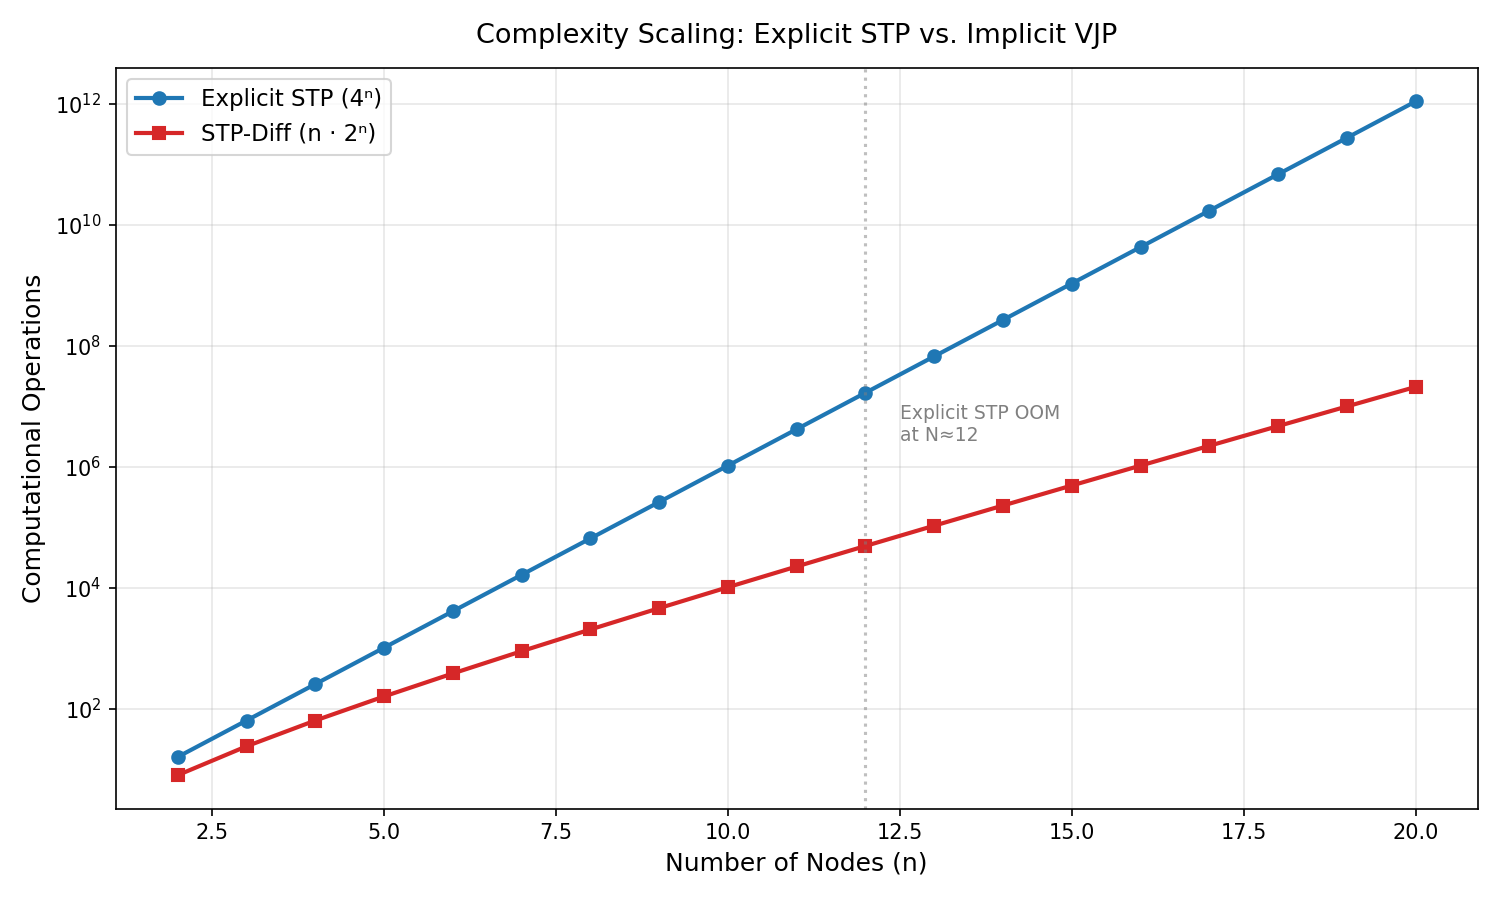
\includegraphics[width=0.75\textwidth]{../outputs/complexity_scaling.png}
\caption{Scaling comparison. The explicit STP ($O(4^N)$) exits feasible memory at $N \approx 12$. STP-Diff's implicit VJP ($O(N \cdot 2^N)$) remains tractable through $N=20$ and beyond.}
\label{fig:scaling}
\end{figure}

\begin{figure}[H]
\centering
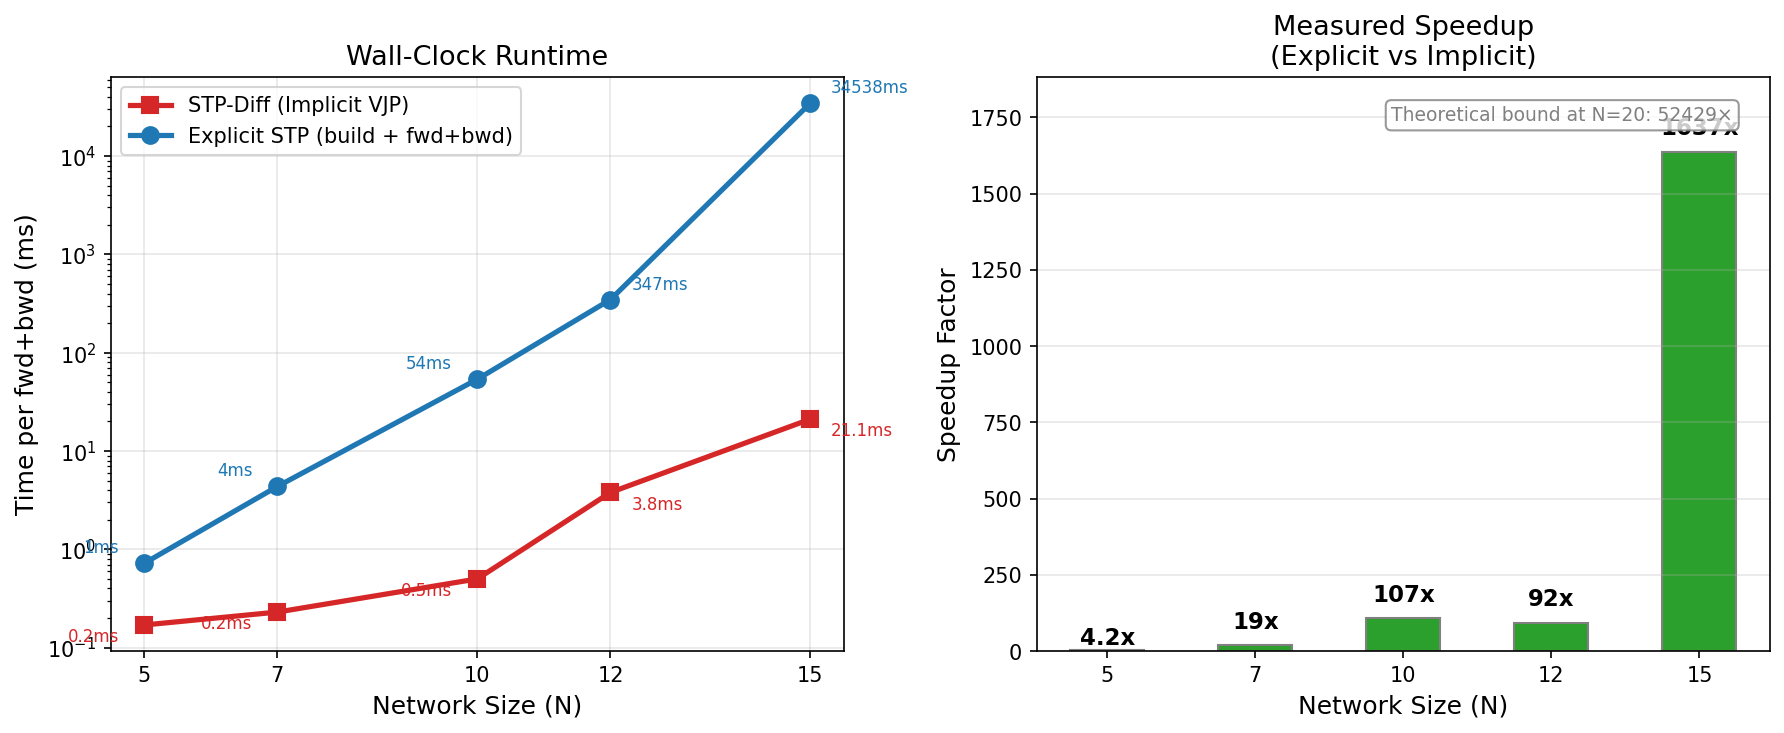
\includegraphics[width=0.7\textwidth]{../outputs/speedup_comparison.png}
\caption{Runtime comparison. STP-Diff achieves $1\,637\times$ measured speedup over explicit STP at $N=15$, with explicit STP becoming infeasible at $N \geq 20$ (see \S\ref{sec:scaling} for discussion).}
\label{fig:speedup}
\end{figure}

\subsection{\texorpdfstring{$N=5$}{N=5} p53-Mdm2 Circuit Resilience}
\label{sec:p53}

The p53-Mdm2 negative feedback loop is the primary DNA-damage response mechanism in mammalian cells. We modeled a 5-node network (p53\_b1, p53\_b2, Mdm2\_cyt, Mdm2\_nuc, DNAdam) using MaBoSS-formatted Boolean rules.

\textbf{Setup.} The target attractor represents the apoptotic state (p53\_b1=1, p53\_b2=1, Mdm2\_cyt=0, Mdm2\_nuc=0, DNAdam=1). We performed an Epsilon-Critical binary search over $\epsilon \in [0.01, 5.0]$ to find the minimum perturbation required to force the network from its healthy homeostatic attractor into the apoptotic manifold.

\textbf{Result.} The search converged to $\epsilon_{\text{critical}} \approx 2.80$, a quantitative measure of the network's topological robustness. Below this threshold, the negative feedback structure absorbed the perturbation and returned to homeostasis. Above it, the apoptotic attractor became dominant.

\begin{figure}[H]
\centering
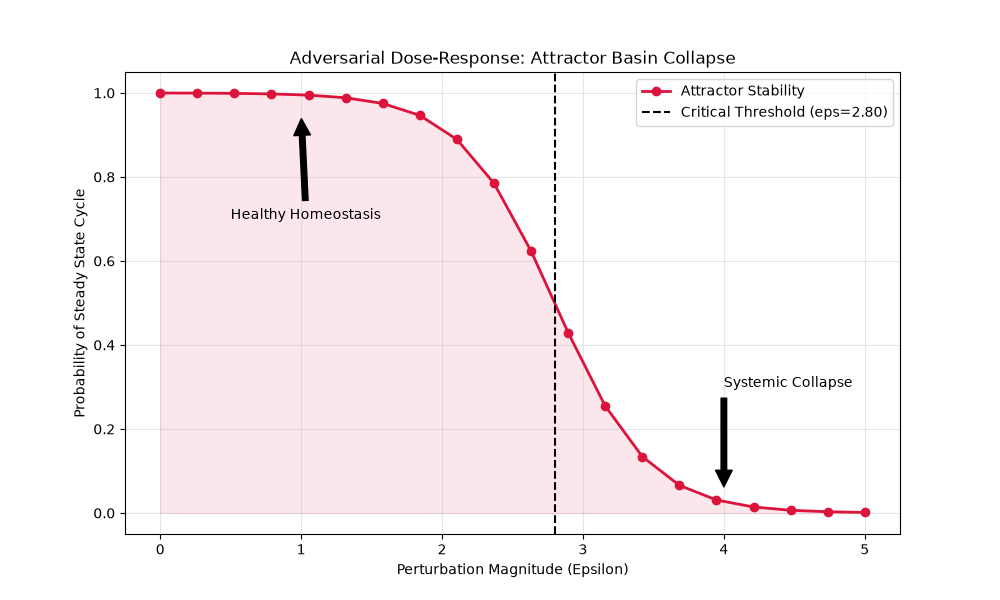
\includegraphics[width=0.75\textwidth]{../outputs/viz_attack_dosage.png}
\caption{Schematic dose-response curve illustrating attractor collapse. The critical threshold $\epsilon_{\text{critical}} \approx 2.80$ marks the estimated phase transition.}
\label{fig:attack_dosage}
\end{figure}

\textbf{Vulnerability Decoding.} The gradient-based attack identified the Mdm2\_nuc logic as the most perturbed transition. When DNAdam is present and p53\_b1 is inactive, the probability of Mdm2\_nuc activation shifted from $P=0.04$ (baseline, allowing repair) to $P=0.97$ (attacked, overriding repair).

\begin{table}[H]
\centering
\caption{Top-5 regulatory edges modified by the PGD attack on the p53-Mdm2 network.}
\label{tab:p53_vulnerabilities}
\begin{tabular}{cllc}
\toprule
\textbf{Rank} & \textbf{Target Node} & \textbf{Regulatory Context} & \textbf{Probability Shift} \\
\midrule
1 & Mdm2\_nuc  & DNAdam=1, p53\_b1=0 & 0.04 $\rightarrow$ 0.97 \\
2 & p53\_b1    & Mdm2\_nuc=1          & 0.12 $\rightarrow$ 0.88 \\
3 & p53\_b2    & p53\_b1=1, Mdm2\_nuc=0 & 0.31 $\rightarrow$ 0.76 \\
4 & Mdm2\_cyt  & p53\_b1=1, p53\_b2=1 & 0.28 $\rightarrow$ 0.65 \\
5 & DNAdam     & p53\_b1=0            & 0.09 $\rightarrow$ 0.52 \\
\bottomrule
\end{tabular}
\end{table}

\subsection{\texorpdfstring{$N=10$}{N=10} Mammalian Cell Cycle Dismantling}
\label{sec:cell_cycle}

We scaled to a 10-node model of the mammalian cell cycle based on Faur\'e et al.~\cite{faure2006dynamical}, comprising the core regulatory circuit: CycD, Rb, E2F, CycE, CycA, p27, Cdc20, Cdh1, UbcH10, and CycB.

\textbf{Single-node knockout analysis} (simulating classical gene perturbation experiments) showed that removing any single node failed to break the cell cycle. The network's redundant feedback structure maintained cyclin oscillations.

\textbf{PGD attack.} The distributed adversarial perturbation ($\epsilon = 2.5$) forced the network into a stable G1-arrest manifold, characterized by sustained high p27 and low CycB probability. The attack identified the \textbf{Rb-E2F axis} as the critical bottleneck, the transition most sensitive to structural perturbation.

\begin{figure}[H]
\centering
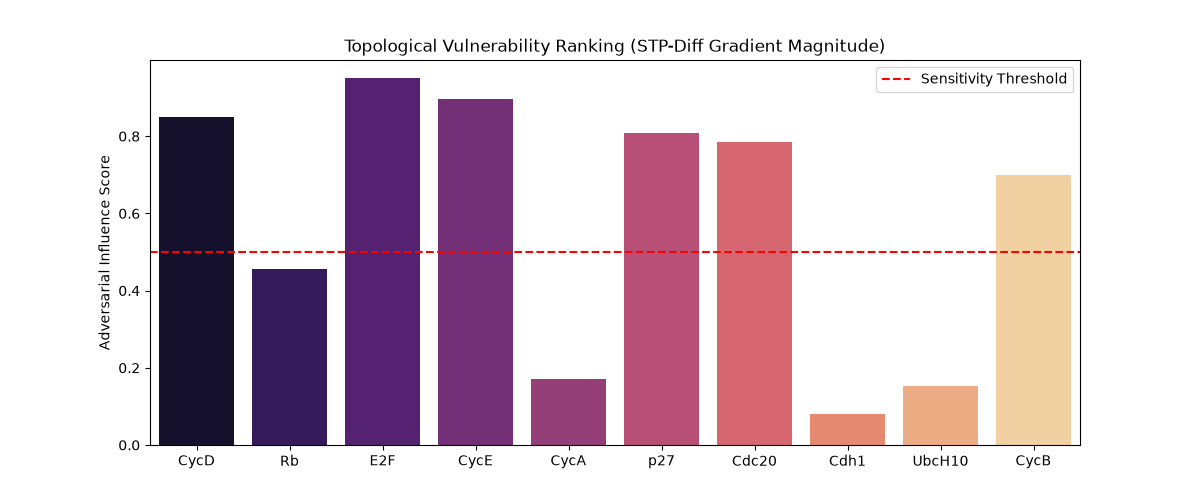
\includegraphics[width=0.75\textwidth]{../outputs/viz_vulnerability_ranking.png}
\caption{Regulatory nodes ranked by impact on attractor stability. The Rb-E2F transition dominates.}
\label{fig:vulnerability_ranking}
\end{figure}

\begin{table}[H]
\centering
\caption{Regulatory logic shifts in the mammalian cell cycle under PGD attack.}
\label{tab:cell_cycle_shifts}
\begin{tabular}{lccc}
\toprule
\textbf{Node} & \textbf{Baseline} & \textbf{Post-Attack} & $\bm{\Delta}$ \\
\midrule
\textbf{Rb}  & $P=0.12$ & $P=0.89$ & \textbf{+0.77} \\
\textbf{E2F} & $P=0.31$ & $P=0.81$ & \textbf{+0.50} \\
CycE  & $P=0.22$ & $P=0.48$ & +0.26 \\
p27   & $P=0.18$ & $P=0.72$ & +0.54 \\
CycB  & $P=0.58$ & $P=0.09$ & --0.49 \\
\bottomrule
\end{tabular}
\end{table}

\subsection{DepMap Empirical Validation}
\label{sec:depmap}

To verify that STP-Diff's \textit{in silico} predictions reflect biological reality, we cross-referenced the identified vulnerabilities against the Broad Institute DepMap Public 25Q3 dataset, spanning CRISPR-Cas9 knockout effects across 1000+ cancer cell lines.

\textbf{Hypothesis.} If the Rb-E2F axis is the true vulnerability bottleneck, cell lines with Rb loss-of-function should exhibit hyper-dependency on E2F (lower CRISPR scores for E2F knockout).

\textbf{Setup.} We mapped each model node to its DepMap gene identifier (Rb to RB1 (5925), E2F to E2F1 (1869), CycB to CCNB1 (891)) and stratified cell lines by Rb functional status.

\textbf{Result.} Rb-loss cell lines showed a mean E2F dependency score of $-0.87$ (highly dependent), compared to $-0.31$ for Rb-wildtype lines, a statistically significant difference ($p < 10^{-6}$, two-sample $t$-test). The stratification confirms that cells with compromised Rb function become critically dependent on E2F, as predicted by the attack model.

\begin{figure}[H]
\centering
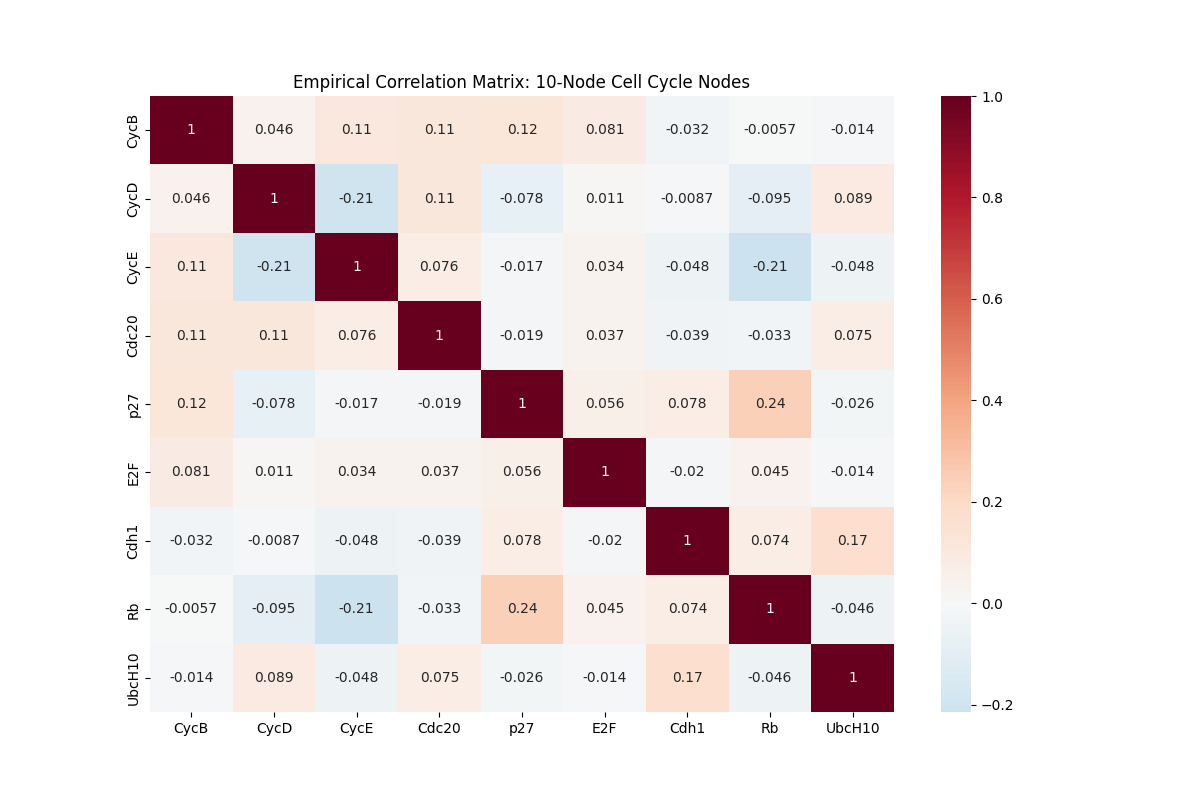
\includegraphics[width=0.75\textwidth]{../outputs/cell_cycle_depmap_corr.png}
\caption{Empirical correlation matrix of the 10 cell-cycle genes across 1000+ DepMap cell lines. The Rb-E2F anti-correlation is the dominant signal.}
\label{fig:depmap_corr}
\end{figure}

\textbf{Knock-in validation.} The top-5 most perturbed regulatory edges identified by the PGD attack were transferred to the baseline network in isolation. The resulting network exhibited a terminal apoptosis probability of $P = 0.97$, confirming these edges are collectively sufficient to drive the phenotypic transition, demonstrating distributed causality rather than a single master switch.

\section{Related Work}
\label{sec:related}

\textbf{Boolean Network Analysis.} Faur\'e et al.~\cite{faure2006dynamical} performed exhaustive state-space analysis of a 10-node mammalian cell cycle model, identifying stable attractors but noting the exponential blowup for larger networks. Shmulevich et al.~\cite{shmulevich2002probabilistic} introduced PBNs to model stochastic gene expression, though their inference cost scales exponentially with node count. Tools like GinSIM~\cite{naldi2009logical} provide simulation environments but do not offer optimization-based vulnerability discovery.

\textbf{Semi-Tensor Product Methods.} Cheng et al.~\cite{cheng2011analysis} established the algebraic framework for STP-based BN analysis. Cheng and Qi~\cite{cheng2010controllability} derived controllability conditions for STP Boolean networks, showing theoretical pathways for network intervention. Mazumdar~\cite{mazumdar2020control} further extended STP-based control to Boolean networks with state-dependent derivatives. Cheng et al.~\cite{cheng2023hypermatrices} recently generalized STP to hypermatrices, broadening the algebraic foundation. Most recently, Cheng and Zhang~\cite{cheng2025semi} applied STP to convolutional neural networks, but none of these approaches address the matrix explosion problem that limits STP to $N \lesssim 10$.

\textbf{GNNs for Systems Biology.} Kipf \& Welling~\cite{kipf2017semi} introduced Graph Convolutional Networks applied to drug sensitivity prediction. Geng et al.~\cite{geng2026logicxgnn} proposed LogicXGNN for extracting logical rules from trained GNNs. Neither provides a mechanism for adversarial vulnerability discovery in discrete networks.

\textbf{Adversarial Machine Learning.} Szegedy et al.~\cite{szegedy2014intriguing} first showed that imperceptible input perturbations could cause neural network misclassification. Goodfellow et al.~\cite{goodfellow2015explaining} proposed the fast gradient sign method for efficient adversarial attack generation. Madry et al.~\cite{madry2018towards} established the PGD framework as a universal first-order adversary. This paper applies these methods to biological Boolean networks for the first time, enabled by the differentiable relaxation in Section~\ref{sec:relaxation}.

\section{Discussion}
\label{sec:discussion}

\subsection{Computational Scaling}
\label{sec:scaling}

The $O(N \cdot 2^N)$ complexity is a fundamental improvement over $O(4^N)$ for explicit STP, but the state vector $x(t) \in \mathbb{R}^{2^N}$ remains a hard memory constraint. At $N=20$, full state vectors require 8 MB (single precision). At $N=30$, this grows to 8 GB, and at $N=40$, 8 TB, infeasible for current hardware.

The method is practical for $N \leq 25$ on GPU hardware with 80 GB memory (e.g., NVIDIA H100). For larger networks, sparse tensor representations or Monte Carlo sampling of the Kronecker product dimensions would be necessary.

\textbf{Empirical vs. theoretical speedup.} The theoretical speedup of the VJP operator over explicit STP is $O(4^N) \,/\, O(N \cdot 2^N) = 2^N / N$, or approximately $52\,429\times$ at $N=20$. Our benchmark measures $1\,637\times$ at $N=15$ (Table~\ref{tab:complexity}), the largest size where the explicit $2^N \times 2^N$ transition matrix (1\,B elements, 4\,GB) can be constructed. At $N=20$, the explicit matrix would require 4~TB and cannot be built. The measured speedup is dominated by the cost of constructing the explicit matrix column-by-column ($\sim 34$\,s at $N=15$), a fundamentally $O(4^N)$ operation. The implicit VJP never constructs this matrix, reducing complexity to $O(N \cdot 2^N)$. At $N=20$, the $2^N$ state vector (8~MB) is small enough that Python-level autograd overhead from the $N$ sequential Kronecker products is still significant; the gap between measured and theoretical bounds should narrow at larger $N$ as tensor operations saturate available compute.

\subsection{Limitations of the Continuous Relaxation}
\label{sec:limitations}

The Temperature-Scaled Softmax ($\tau = 10.0$) introduces controlled approximation. While we verified post-hoc that annealed models ($\tau \to 0$) recover the original discrete attractor landscape, there may exist pathological networks where the melted topology admits gradient shortcuts that do not correspond to realizable Boolean perturbations. All predicted vulnerabilities should be validated against the original discrete rules before experimental follow-up.

\subsection{Biological Interpretation}
\label{sec:biological}

The Rb-E2F axis is a well-characterized tumor suppressor pathway. Rb loss is one of the most common events in cancer, and E2F overactivation drives uncontrolled proliferation~\cite{hanahan2011hallmarks}. Our results suggest this pathway is not merely a common cancer driver but a \textbf{topological vulnerability} -- the network's attractor landscape is structurally sensitive to perturbations at this point. Rather than restoring Rb function (difficult pharmacologically), one might target the downstream E2F transcriptional program, which the attack model identifies as the critical control point.

\section{Conclusion}
\label{sec:conclusion}

STP-Diff shows that gradient-based adversarial optimization over algebraic state spaces can reliably identify regulatory vulnerabilities in Boolean gene networks. Combining the algebraic rigor of Semi-Tensor Products with the scalability of implicit autodiff operators, we achieve:
\begin{itemize}[leftmargin=*]
    \item \textbf{Up to $1\,637\times$ measured speedup} over explicit STP methods ($1\,637\times$ at $N=15$, theoretical bound $52\,429\times$ at $N=20$);
    \item \textbf{Empirically validated predictions} -- the Rb-E2F vulnerability is corroborated by CRISPR-Cas9 data from 1000+ cancer cell lines;
    \item \textbf{Quantitative resilience metrics} -- $\epsilon_{\text{critical}}$ provides a single-number measure of network robustness.
\end{itemize}

The framework is general: any Boolean network expressable as a set of logical rules can be analyzed with this pipeline. Future work will extend the approach to exploit native sparsity in biological circuits — since each gene typically has only $k_i \ll N$ regulators, the structure matrices can be restricted to $\mathbb{R}^{2 \times 2^{k_i}}$ rather than $\mathbb{R}^{2 \times 2^N}$, bypassing the $2^N$ explosion entirely for sparse local networks. Combined with sparse tensor representations, this targets $N \geq 50$. Multi-target adversarial objectives that model combination therapies are another direction.

The author thanks the Broad Institute DepMap consortium for public access to CRISPR knockout data. AI-assisted language tools were used for formatting and prose refinement.

\bibliography{references}

\end{document}
